\chapter{Реализация серверной части}
\section{Проектирование нейросетевой части приложения}
В рамках разделенной структуры сервисов для реализации необходимого функционала системы было принято решение написать функциональные интерфейсы для обученной нейросетевой модели. 

Подход к имплементации архитектуры сети позволял выбирать из множества различных решений. Многие из типовых архитектур позволяют строить не только отображения множества реплик в множества ответов, но также строят языковую модель и семантическое ядро текста. Полнофункциональные модели различных архитектур нейронных сетей имеют множетсво параметров, что в данном случае является избыточным. 

Было принято решение имплементировать реккурентные типы нейронных сетей, используя типовые архитектуры для генерации по примеру зарубежных коллег \cite{li2016deep, sharma2016natural,толкачев2019нейронное}. Использованные ими различные походы к язковому моделирования диалогов помогли с выбором арзитектуры ячеек сети и подготовкой набора данных для обучения. 

Для реализации была выбрана двунаправленная сеть долгой-короткой памяти (bidirectional Long-Short Time Memory network). Языком для реализации послужил Python 3 и набор необходимых библиотек для обучения нейронных сетей.

Для успешного обучения сети необходим качественный и хорошо подготовленный, обширный набор данных. Для целевого домена сети (психология) на момент написания выпускной квалификационной работы открытых наборов данных не существовало. Более того, существующие наборы данных на русском языке для более широкого семантического домена (диалоги) также не позволяли провести успешное обучение диалогового агента. 

Обучение сети проводилось на базе сервиса Colaboratory от компании Google. Сервис предоставляет бесплатные вычислительные мощности для исследователей и студентов в рамках учебных проектов. Colaboratory имеет удобный интерфейс и позволяет запускать фоновые задачи для обучений нейросетевых моделей. Испанские исследователи более подробно описывают функционал сервиса и проводят анализ и сравнение с аналогами \cite{carneiro2018performance}.

Перед обучением сети необходимо подготовить набор данных. Поскольку набор данных необходимо еще было собрать, было принято решение использовать в качестве источника диалогов между двумя коммуникационными агентами смешанный набор из выделенных частей субтитров с сайта Open Subtitles, как это было сделано в работах \cite{creutz2018open, arcan2016asistent} и выделенных из текстов пьес диалогов из открытых источников. 

Перед тем как добавить диалоги из субтитров необходимо было выделить их из файлов субтитров. Для этого был написан скрипт автоматизации экстракции содержимого субтитров. Скрипт извлекает и сортирует содержимое на токены, в данном случае токенами служат приложения. После чего они очищаются от непечатных и иных не поддерживаемых символов, стоп слов. Пример листинга скрипта представлен на листинге \ref{listing:1}, в целом скрипт представляет собой простой класс-обработчик вызываемый при запуске скрипта. 

\begin{listing}[H]
\inputminted[breaklines, breakanywhere, linenos, fontsize=\small]{python}{source/prepare_subtitles.py}
\caption{Часть скрипта обработки субтитров}
\label{listing:1}
\end{listing}

После пред-обработки субтитров, файл отправляется на токенизацию вида <<Вопрос – Ответ>>. Очищенные данные разбиваются на строки и распределяются в два файла. Следующим этапом является разбиение на обучающую и тестовую выборки и выравнивание входящих последовательностей. Листинг кода функций выравнивания представлен на листинге \ref{listing:2}. На этом этапе возможно построение гистограммы длин всех последовательностей ля визуального анализа. Гистограмма размеров представлена на рисунке \ref{fig:len}. 

\begin{listing}[H]
   \inputminted[breaklines, breakanywhere, linenos, fontsize=\small]{python}{source/padding.py}
\caption{Функции реализующие выравнивание входящих последовательностей}
\label{listing:2}
\end{listing}

Далее необходимо преобразовать токены слова сначала в мешок слов. Процесс преобразования включает в себя построение индекса слов, их числового представления распределенного по частоте встречаемости \cite{zhao2017bagwords}. Сформировав индекс возможно построение модели word2vec отображающей множество слов в множество их векторных представлений.

Word2Vec — это набор алгоритмов для расчета векторных представлений слов \cite{word2vecproject}.Он принимает текстовый корпус в качестве входных данных и, после получения словаря из обработанных текстовых материалов, образует векторы слов на выходе. Принцип работы состоит в нахождении связей между контекстами слов, ведь слова, находящиеся в похожих контекстах, часто могут быть семантически близкими. То есть нужно максимизировать косинусную близость между векторами слов, появляющихся в близких контекстах, и минимизировать косинусную близость слов, не появляющихся в контексте друг друга \cite{word2vecproject}. 

При обучении нейронной сети одним из подходов является <<Skip-gram>>, где каждое слово заменяется номером его семантической группы, что позволяет получить <<мешок>> слов с глубоким смыслом, избегая потери учета семантики слова — предсказывается контекст при данном слове. Эти взвешенные векторы фиксированной длины для каждого слова объединяются, используя алгоритм кластеризации (k-средних) \cite{mikolov2013distributed, левченко2017разработка}.

\begin{figure}[H]
    \centering
    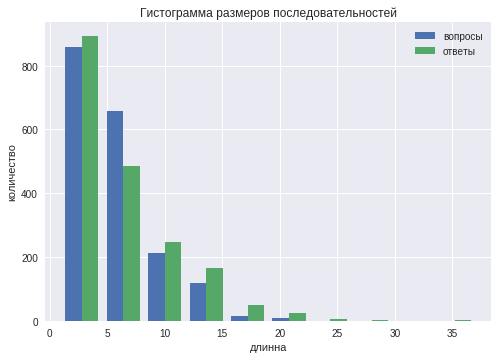
\includegraphics[width=0.8\textwidth]{image/hist_len.png}
    \caption{Гистограмма длин }
    \label{fig:len}
\end{figure}

Готовые векторные представления подаются на вход нейронной сети для обучения. Как уже было сказано ранее сеть имеет архитектуру <<bidirectional LSTM>>. Двунаправленные рекуррентные нейронные сети (bi-LSTM) \cite{hochreiter1997lstm} были разработаны для кодирования каждого элемента в последовательности с учетом левого и правого контекстов, что делает их одним из лучших вариантов для решения задачи распознавания именованных сущностей. 

Двунаправленный расчет модели состоит из двух этапов: прямой слой вычисляет представление левого контекста, и обратный слой вычисляет представление правого контекста. Выходы этих шагов затем объединяются для получения полного представления элемента входной последовательности. Было показано, что bi-LSTM полезны во многих задачах естественного языка, таких как машинный перевод, ответ-вопросные системы и особенно в распознавании именованных сущностей. Для реализации интересен именно аспект вопросно-ответных систем \cite{распознаваниесущностей}. 

Для имплементации архитектуры представленной на рисунке \ref{fig:lstm} использовалась библиотека Keras \cite{keras}. Библиотека предоставляет обширные функциональные возможности для проектирования самых разных нейронных сетей, а так же утилиты для подготовки данных, сортировки и другие возможности. Для упрощения проектирования сети использовалась библитека seq2seq \cite{Britz:2017} позволяющая импортировать уже готовые типовые структуры ячеек и сосредточится на настройке поток данных и гиперпараметрах. Обучение сети длилось более 10 часов на мощностях сервиса Colaboratory. 

\begin{figure}[H]
    \centering
    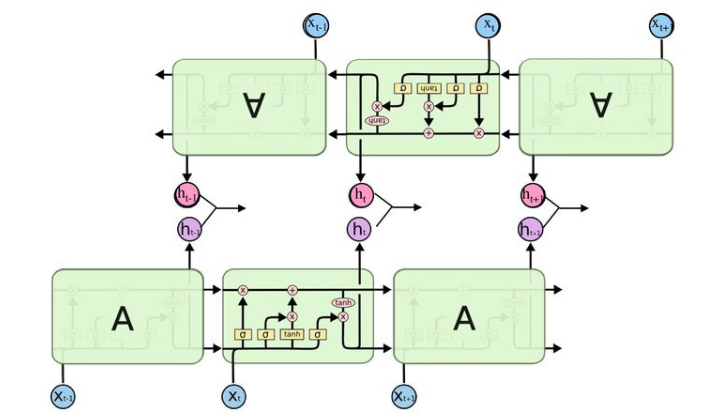
\includegraphics[width=0.8\textwidth]{image/bi-LSTM.png}
    \caption{Архитектура bi-LSTM}
    \label{fig:lstm}
\end{figure}

Пример листинга кода построения модели сети на Keras приведен на листинге \ref{listing:3}. Построение модели представляет собой последовательное дополнение структурного графа вычислений который перед исполнением передается библиотеке Tensorflow для перевода в оптимизированный код на языке C.  

\begin{listing}[H]
\inputminted[breaklines, breakanywhere, linenos, fontsize=\small]{python}{source/keras.py}
\caption{Построение архитектуры модели нейронной сети}
\label{listing:3}
\end{listing}

Настроив цикл обучения на тестовый вывод каждой сотой эпохи обучения, получим следующий вывод на этапах обучения, представленный на рисунке . В вывод отображается эпоха, текущая батч-свертка, время, величина потери сети и выходные значения некоторого тестового примера из выборки. Вывод консоли представлен ниже:


\begin{minipage}{0.9\textwidth}
   
        \begin{minted}[breaklines, breakanywhere, fontsize=\small]{pycon}
        Training epoch: 4000, training examples: 10626 - 21252
        Epoch 1/1
        82267/82267 [==============================] - 734s 9ms/step - loss: 0.1241
        . что что это значит не делает ? end end что сейчас ? end end что они ? end end что end все end end всё это end end что 
        \end{minted}
    
\end{minipage}\\[1.5pt]


Постепенно нейронная сеть стремится к уменьшению значения потерь пока они не дойдут до указанного минимума, в данном случае установлено, что \mintinline{python}{ ad = Adam(lr=0.00005) } это значит обучение закончится тогда, когда значение потерь станет равным указанному числу. 

После обучения сети необходимо было написать функции-интерфейсы к обьекту модели для использования в приложении Django. В результате обучения сеть способна вести диалоги с контекстной длиной в одну фразу и готова к использованию в проектах. 

\section{Проектирование приложения на фреймворке Django}
Один из самых простых и незамысловатых способов создать веб-приложение на Python с нуля – это воспользоваться стандартом Common Gateway Interface (CGI), который приобрел популярность примерно в 1998 году. Но с развитием веб-стандартов и протоколов обычное приложение CGI уже не удовлетворяет требованиям пользователей. 

Возникает необходимость в гибком подходе к проектированию функциональных веб-приложений. Фреймворк Django спроектирован для решения таких задач. Приложения для фреймворка проектируются по паттерну Модель-Отображение-Контроллер (MVC) при котором за различные части приложения отвечают различные части программного кода. 

Модели представляют обьекты которые хранятся в базе данных приложения. В файле <<models.py>> производится перечисление всех абстракций обьектов с которыми необходимо работать в хранилище и в классе каждого объекта определяются поля обьекта и отношения между ними. На листинге 2.\ref{listing:4} представлен пример обьекта-модели проектируемого приложении. 

\begin{listing}[H]
\begin{minted}[breaklines, breakanywhere, linenos, fontsize=\small]{python}
class Message(models.Model):
    """
    Класс экземпляра  сообщения в чате
    """
    id_chat = models.ForeignKey(Chat, on_delete=models.CASCADE)
    date = models.DateTimeField(auto_now_add=True)
    text = models.TextField()
    id_user = models.ForeignKey(User, on_delete=models.CASCADE)

    def __str__(self):
        return str(self.id)

\end{minted}
\caption{Пример модели приложения}
\label{listing:4}
\end{listing}

Внутри класса объекта представлены несколько полей. Два из них являются зависимыми к другим таблицам по типу <<многие-к-одному>> к другим моделям. Ключевой аргумент \mintinline{python}{on_delete = models.CASCADE} позволяет удалять все связанные записи каскадно. Другие поля представляют собой поля типа <<дата/время>> и поле для хранения текста без форматирования. 

В комплекте Django есть модуль Django ORM который реализует работу с различными базами данных, генерируя запросы, таблицы и реляций в полуавтоматическом режиме. 

Настройки базы данных, как и многие другие настройки приложения Django определяются в файле <<settings.py>>. Ниже представлен фрагмент листинга файла приложения: 

\begin{minipage}{0.9\textwidth}
        \begin{minted}[breaklines, breakanywhere, fontsize=\small]{python}
        # Database
        # https://docs.djangoproject.com/en/2.1/ref/settings/#databases
        
        DATABASES = {
            'default': {
                'ENGINE': 'django.db.backends.sqlite3',
                'NAME': os.path.join(BASE_DIR, 'db.sqlite3'),
            }
        }
        \end{minted}
\end{minipage}\\[1.5pt]

Для окружения разработчика используется СУБД <<SQLite>>. Это легковесная встраиваемая СУБД в формате C-библиотеки позволяет выстраивать окружение разработчика без установки дополнительных инструментов управления конфигурацией СУБД.

Структура базы данных приложения представлена на рисунке \ref{fig:db}.

\begin{figure}[H]
    \centering
    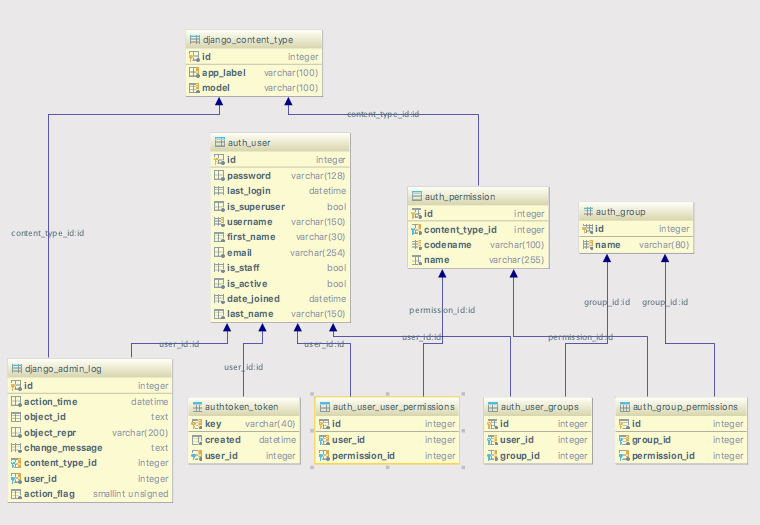
\includegraphics[width=0.9\textwidth]{image/db_diagram.png}
    \caption{Структура базы данных приложения}
    \label{fig:db}
\end{figure}

Django позволяет создавать веб-приложение, но в соотвествии со структурой проектируемого приложения необходимо предоставить клиентской части API для работы. В качестве стандарта используется стандарт соглашения о REST структуре \cite{richardson2008restful}. Для реализации  REST-апи используется библиотека <<Django REST Framework>> (DRF). 

Для работы DRF необходимо создать файлы сериализации моделей, а также файл в котором будут отбражены правила взаимодействия и вызываемые функции в процессе работы с интерфейсами приложения. 

Ниже приведен пример листинга файла <<serializer.py>>:

\begin{minipage}{0.9\textwidth}
        \begin{minted}[breaklines, breakanywhere, fontsize=\small]{python}
        from rest_framework import serializers

        from psiChat.models import Dialogue
        
        
        class DialogueSerializer(serializers.HyperlinkedModelSerializer):
            class Meta:
                model = Dialogue
                fields = ('id','name', 'description', 'number_steps',)

        \end{minted}
\end{minipage}\\[1.5pt]

В начале скрипта импортируется модель которой необходим интерфейс для сериализации в JSON и обратно. После чего создается класс наследуюемый от класса <<HyperlinkedModelSerializer>>. В мета-классе, который при выполнении интерпретатор преобразует в свойства класса и вызовы функций, определяем поля которые необходимо сереализовать. В примере представлен типовой сериалайзер для модели который предоставляет готовые автоматически сгенерированные функции для различных вызовов. 

После создания сериалайзера для работы приложения необходимо создать ее представление. Для этого рассмотрим скрипт <<dialigue.py>> (листинг 2.\ref{listing:5}) в котором определено представление модели через типовой класс DRF -- ModelViewSet. В начале скрипта импортируем необходимые объекты и функции. Определяем размер выборки из базы данных при помощи свойства класса <<queryset>>. Так же определим классы доступа к представлению модели при помощи свойства <<permissions\_classes>>, для всех пользователей. 

\begin{listing}[H]
\begin{minted}[breaklines, breakanywhere, linenos, fontsize=\small]{python}
    from rest_framework import viewsets
    import rest_framework.permissions as permissions
    from psiChat.models import Dialogue
    from psiChat.serializers import DialogueSerializer
    
    
    class DialogueViewSet(viewsets.ModelViewSet):
        queryset = Dialogue.objects.all()
        serializer_class = DialogueSerializer
        permissions_classes = [permissions.AllowAny]
        def get_queryset(self):
            """
            This view should return a list of all records
            """
            return Dialogue.objects.all().order_by('name')

\end{minted}
\caption{Пример представления модели для API}
\label{listing:5}
\end{listing}

Закончить подготовку АПИ можно сформировав необходимые сериализаторы и представления и далее просто определить их адреса через типовой класс <<router>> предоставляемый DFR. 

\section{Интеграция модели Tensorflow в приложение Django}
Следующей задачей небходимой для реализации программы является интеграция сформированной в пункте 2.1 модели нейронной сети. 

Существующие решения (например, <<TensorFlow Serve>>) для интеграции не предоставляют достаточной гибкости и требуют обслуживания и развертывания дополнительных сервисов для работы. Было принято решение интегрировать модель как модуль для вызова во время запуска Django-приложения. 

Для выполнения этой задачи необходимо произвести специализированную настройку графа вычислений при запуске Django. Во время запуска необходимо проихвести <<заморозку>> и импортирование единственного графа вычиcлений. Объявим переменные хранящие путь до сохранненной обученной модели и векторным представлениям слов. Реализация этой задачи представлена ниже: 

\begin{minipage}{0.9\textwidth}
        \begin{minted}[breaklines, breakanywhere, fontsize=\small]{python}
        filename_net_model = os.path.join(BASE_DIR, 'psiChat/chatModule/chitchat/data/net_model.txt')
        filename_net_weights = os.path.join(BASE_DIR, 'psiChat/chatModule/chitchat/data/net_final_weights.h5')
        filename_w2v_model = os.path.join(BASE_DIR, 'psiChat/chatModule/chitchat/data/w2v_model.bin')
        pr = Prediction(filename_net_model=filename_net_model,
                        filename_net_weights=filename_net_weights,
                        filename_w2v_model=filename_w2v_model)
        global graph
        graph = tensorflow.get_default_graph()
        MODEL = pr
        \end{minted}
\end{minipage}\\[1.5pt]

Выполнив все выше перечисленные действия можно спроектировать и запрограммировать серверную часть приложения с интегрированной предобученной моделью Tensorflow.


